%!TEX root = ../thesis.tex
%*******************************************************************************
%****************************** Second Chapter *********************************
%*******************************************************************************

\chapter{Compatible Pants Decomposition for Punctured Surfaces following Gallo-Kapovich-Marden}

Let $S_{g,n}$ be a genus $g$ surface with $n$ punctures, $(g,n) \geq (1,1)$, then there exists essential simple closed curves $a_1, b_1, \ldots, a_g, b_g$ and peripheral simple closed curves $c_1, \ldots, c_n$ such that 
\[\pi_1(S_{g,n},p) = \Bigg \langle a_1, b_1, \ldots,,a_g, b_g, c_1, \ldots, c_n \Bigg \vert \left(\prod_{i=1}^{g}b_i^{-1}a_i^{-1}b_i a_i \right) c_1 \ldots c_n \Bigg \rangle,\]
\[i(a_i,b_i) = 1, i(a_i,a_j) = i(b_i,b_j)=i(a_i,b_j)= i(a_i,c_l) = i(b_i,c_l) = i(c_l,c_k)= 0, \] 
\[a_i \cap b_i = b_i \cap b_j = a_i \cap b_j = a_i \cap c_l = b_i \cap c_l = c_l \cap c_k = \{p\}, \]
\[\forall i \neq j, k \neq l, i,j \leq g \text{ and } k,l\leq n\]

Here, $i(a, b)$ denotes the minimum number of intersections between the curves in the isotopy classes of $a$ and $b$, which is called the \textit{geometric intersection number}.

    \begin{figure}[h]
	\labellist	
	
	\pinlabel $a_1$ at 55 160 
	\pinlabel $b_1$ at 120 225 
	\pinlabel $a_2$ at 220 70
	\pinlabel $b_2$ at 320 225
	
	\pinlabel $c_1$ at 460 200 
	\pinlabel $c_2$ at 460 120
	\pinlabel $c_3$ at 460 40 
     \endlabellist
     \centering
	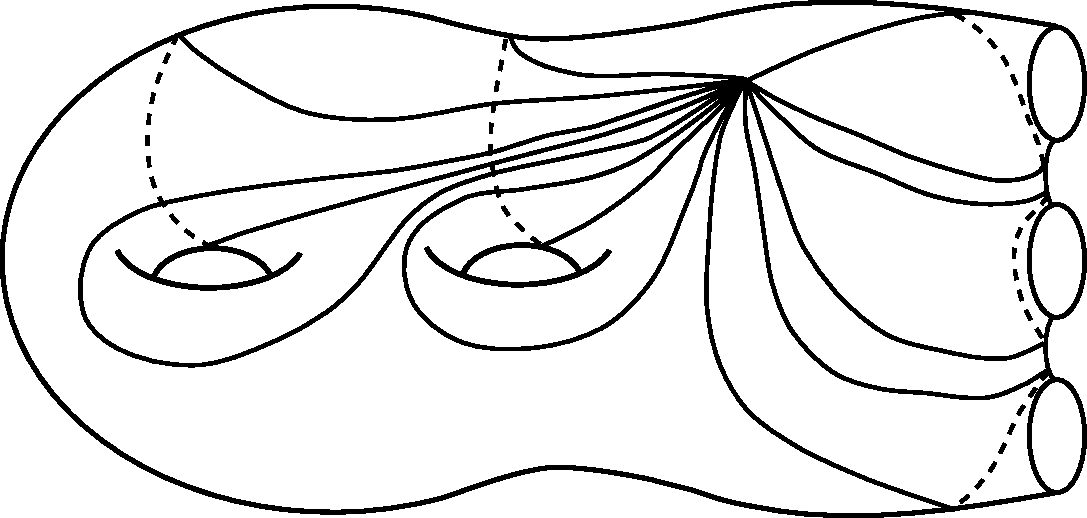
\includegraphics[width=8cm]{Chapter2/Figs/fund_group}
	\caption{Generators of $\pi_1(S_{g,n})$}
	\label{fig:Gen}
    \end{figure}    


\begin{defn}\label{defn:handle}
	Let $\rho: \pi_1(S_{g,n},p) \rightarrow \pslc$ be a representation. A \textit{handle} $H$ of $S$ is defined as a set of two simple closed curves $a, b$ such that:
	\begin{enumerate}
		\item $a \cap b = \{p\}$ and $i(a,b) = 1$.
		\item $\rho(a)$ and $\rho(b)$ are loxodromic.
		\item The subgroup generated by $\rho(a)$ and $\rho(b)$ i.e., $\langle \rho(a), \rho(b) \rangle$ is non-elementary.
	\end{enumerate}
\end{defn}


\begin{theorem}
	Let $S_{g,n}$ be a genus $g$ surface with $n$ punctures and $p$ be a fixed basepoint on $S$. Let $\rho: \pi_1(S_{g,n},p) \rightarrow \pslc$ be a non-elementary representation such that $\rho(c_j)$ is loxodromic for every $j$. Then, there exists a family of $3g - 3 + n$ essential simple closed curves $\Gamma \coloneqq \{\gamma_1, \ldots, \gamma_{3g-3+n}\}$ such that $S_{g,n} \setminus \Gamma = \bigsqcup_{i=1}^{2g-2+n} P_i$, where each $P_i$ is a pair of pants such that $\rho|_{P_i}$ is Schottky.
\end{theorem}

The case when $n=0$ is dealt in \cite{GKM}. The proof of the theorem has three steps:
\begin{enumerate}
	\item Firstly, the existence of a handle is proved by using elementary lemmas from plane hyperbolic geometry. We follow the proof of \cite{GKM} with minor modifications to fit to the case of surfaces with punctures. The proof is divided into four cases. 
	
	The first (second resp.) case deals with finding a handle when there exists a simple non-separating curve which is loxodromic (parabolic resp.). These cases are proved exactly as in \cite{GKM}, except for easy checks whether the curves we form using concatenations would still satisfy the required properties. This is required because, in surfaces with punctures we have peripheral curves which behave slightly differently than the non-peripheral ones (see \ref{proof:case1}, \ref{proof:case2}). 
	
	The rest of the cases are proved by reducing to the first and second cases i.e., by finding a non-separating simple closed curve that goes to a loxodromic or parabolic. The interesting situation that occurs in the case of surface with punctures is when $\rho(a_i)=\rho(b_i)=\text{Id}, \forall 1 \leq i \leq g$ (see \ref{proof:case4}). For this to occur, there should be atleast three punctures, otherwise the representation would be elementary. We find the appropriate handle by concatenating the peripheral curves with suitable $a_i$s, $b_i$s and applying hyperbolic plane geometry lemmas on them. 
	
	Note that in Section~\ref{sec:HandleExistence}, we don't assume that peripheral curves go to loxodromics. This step is valid for any non-elementary representation.
		
	\item The second step is to inductively construct a handle and a disjoint non-separating simple closed loxodromic and to cut along this loxodromic to get a surface with genus decreased by 1 and number of boundaries increased by 2. At the end of this step, we will be left with a torus with $2(g-1)+n$ boundary components. From \cite[Section 4]{GKM}, this step also doesn't require the assumption that peripheral curves go to loxodromics under the representation.
	
	\item The final step is to find separating simple closed loxodromics  such that when we cut along them we get a pair of pants with Schottky representation. To follow the proof exactly as in \cite{GKM}, we need to assume that peripheral curves go to loxodromics. 
\end{enumerate}

\section{Existence of a Handle}\label{sec:HandleExistence}
From now on, we will denote $S_{g,n}$ by $S$ for brevity. We denote by $\fxp{\alpha}$, the fixed points of a M{\"o}bius transformation $\alpha$.
\begin{prop}
	Given a non-elementary representation $\rho:\pi_1(S,p) \rightarrow \pslc$, there exists a handle. 
\end{prop}
This proposition is proved in \cite{LeFils}. We give more details and this exposition is analogous to the proof in \cite{GKM}. 

\subsection{Case 1}  \label{proof:case1} Suppose there exists a simple non-separating curve $a$ such that $\alpha \coloneqq \rho(a)$ is loxodromic. There exists $b \in \pi_1(S,p)$ such that $a \cap b = \{p\}$ and $i(a,b) = 1$. Denote $\rho(b)$ by $\beta$.
\subsubsection{Case 1(a)} \label{proof:case1a} Suppose $\fxp{\alpha} \cap \fxp{\beta} = \emptyset$ and $\beta$ does not interchange elements of $\fxp{\alpha}$. We can assume, after conjugating with an appropriate element that 
\[\alpha = \begin{pmatrix}
	\lambda & 0 \\
	0 & \lambda^{-1}
\end{pmatrix}, 
\beta = \begin{pmatrix}
	a & b\\
	c & d
\end{pmatrix},\]
where $|\lambda|>1$ and $ad - bc = 1$. Now, we look at the matrix $\beta \alpha^k$ which is given as follows:
\[\beta \alpha^k = 
	\begin{pmatrix}
		a & b\\
		c & d
	\end{pmatrix} 
	\begin{pmatrix}
		\lambda^k & 0 \\
		0 & \lambda^{-k}
	\end{pmatrix} = 
	\begin{pmatrix}
		a \lambda^k & b \lambda^{-k} \\
		c \lambda^k & d \lambda^{-k}
	\end{pmatrix}
\]

Note that $|\tra(\beta \alpha^k)| = |a \lambda^k + d \lambda^{-k}|$. From our assumptions, we get that $a$ and $d$ both cannot be zero, thus, there exists a $k$ such that $\beta \alpha^k$ is loxodromic. Also, it is easy to note that $\langle \alpha, \beta \alpha^k \rangle$ is non-elementary. Thus, $a$ and $b a^k$ satisfy all the three conditions of the Definition~\ref{defn:handle}

\subsubsection{Case 1(b)} \label{proof:case1b} Suppose $\fxp{\alpha} \cap \fxp{\beta} = \{O\}$. There exists a simple closed curve $y \in \pi_1(S,p)$ such that $\rho(y)(O) \neq O$ and $i(y,a)= i(y,b) = 0$. Suppose not, then $O$ would be fixed by every element in $\rho(\pi_1(S, p))$ making the representation elementary. Now, denote $\rho(y) $ by $\eta$ and orient $y$ in such a way that $ay$ becomes a simple closed curve. Also, note that $i(ay, ba^k) = 1$, for all $k$. 

Now, we prove that there exists $k$ such that $\beta \alpha^k$ and $\alpha \eta$ have the properties of $\alpha$ and $\beta$ as in the Case~\ref{proof:case1a}, respectively. We can assume, after conjugating with an appropriate element that 
\[\alpha = \begin{pmatrix}
	\lambda & 0 \\
	0 & \lambda^{-1}
\end{pmatrix}, 
\beta = \begin{pmatrix}
	a & b\\
	c & d
\end{pmatrix},\]
where $|\lambda|>1$ and $ad - bc = 1$. Now, we look at the matrix $\beta \alpha^k$ which is given as follows:
\[\beta \alpha^k = 
\begin{pmatrix}
	a & b\\
	c & d
\end{pmatrix} 
\begin{pmatrix}
	\lambda^k & 0 \\
	0 & \lambda^{-k}
\end{pmatrix} = 
\begin{pmatrix}
	a \lambda^k & b \lambda^{-k} \\
	c \lambda^k & d \lambda^{-k}
\end{pmatrix}
\]

Now, either $\beta(0) = 0$ or $\beta(\infty)=\infty$, this implies that $b = 0$ or $c = 0$, which in turn implies that $a \neq 0$ or $d \neq 0$. Also, $|\tra(\beta \alpha^k)| = |a \lambda^k + d \lambda^{-k}|$. Thus, there exists $k$ such that $\beta \alpha^k$ is loxodromic.

Let $q \in \fxp{\alpha \eta}$ and suppose $\beta \alpha^k(q) = \beta \alpha^{k+m}(q) = q$ for some $k, m \neq 0$. This implies that $\alpha^m(q)=q$, which in turn says that $q \in \fxp{\alpha}$, as $\alpha$ is loxodromic. This also implies that $q \in \fxp{\beta}$, therefore $q = O$. Now, $\alpha \eta(O) = O \iff \eta(O) = O$, which is a contradiction. Therefore, $\alpha \eta$ can share a fixed point with $\beta \alpha^k$ for atmost one $k$.

Now, suppose $q \coloneqq \alpha \eta(O) \in \fxp{\beta \alpha^k} \cap \fxp{\beta \alpha^{k+m}}$, this again implies that $q \in \fxp{\alpha}$ and thus $q \in \fxp{\beta}$. Therefore, $q = O$, which is a contradiction. Therefore, $\alpha \eta$ can interchange fixed points of $\beta \alpha^k$ for atmost one $k$. Hence, there exists $k$ such that, $\fxp{\beta \alpha^k} \cap \fxp{\alpha \eta} = \emptyset$ and $\alpha \eta$ does not interchange the fixed points of $\beta \alpha^k$ bringing us to the Case~\ref{proof:case1a} 

\subsubsection{Case 1(c)} \label{proof:case1c} Suppose $\beta(\fxp{\alpha}) = \fxp{\alpha}$. There exists a simple closed curve $y \in \pi_1(S,p)$ such that $i(y,a) = i(y,b)=0$ and $\rho(y)(\fxp{\alpha}) \neq \fxp{\alpha}$. Now, orient $y$ such that $yb$ is a simple closed curve such that $a \cap yb = \{p\}, i(a, yb)= 1$. Denote $\rho(y)$ by $\eta$. Suppose that $\eta \beta(\fxp{\alpha}) = \fxp{\alpha}$, this implies that $\eta(\fxp{\alpha}) = \fxp{\alpha}$ which is a contradiction. Therefore, $\eta \beta$ neither interchanges the fixed points nor shares a fixed point with $\alpha$, bringing us to Case~\ref{proof:case1a} or it shares a fixed point with $\alpha$, bringing us to Case~\ref{proof:case1b}.

\subsection{Case 2}\label{proof:case2} Suppose there exists a simple non-separating curve $a$ such that $\alpha \coloneqq \rho(a)$ is parabolic. Again, there exists $b \in \pi_1(S,p)$ such that $a \cap b = \{p\}$ and $i(a,b) = 1$. Denote $\rho(b)$ by $\beta$.

\subsubsection{Case 2(a)}\label{proof:case2a} Suppose $\fxp{\alpha} \cap \fxp{\beta} = \emptyset$. We can assume after conjugating with an appropriate element that 
\[\alpha = \begin{pmatrix}
	1 & 1\\
	0 & 1
\end{pmatrix}, 
\beta = \begin{pmatrix}
	a & b\\
	c & d
\end{pmatrix},
\]
where $ad-bc=1$. Now,

\[\beta \alpha^k = \begin{pmatrix}
	a & b\\
	c & d
\end{pmatrix}
\begin{pmatrix}
	1 & k\\
	0 & 1
\end{pmatrix} = \begin{pmatrix}
	a & ka+b\\
	c & kc+d
\end{pmatrix}\]

Note that, $|\tra{\beta \alpha^k}| = |a + kc + d|$. From our assumptions about the fixed points, we get that $c \neq 0$. Therefore, for large enough $k$ we have that $\beta \alpha^k$ is loxodromic. Now, as $ba^k$ is a non-separating simple closed curve, we go back to Case~\ref{proof:case1}.

\subsubsection{Case 2(b)}\label{proof:case2b} Suppose $\fxp{\alpha} \cap \fxp{\beta} = \{O\}$. There exists a simple closed curve $y \in \pi_1(S,p)$ such that $i(y,a) = i(y,b) = 0$ and $\eta \coloneqq \rho(y)$ does not fix $O$. Now orient $y$ such that $yb$ represents a simple closed curve this implies that $yba^k$ also represents a simple closed curve. Now, as $\eta \beta (O) = \eta(O) \neq O$, we go back to Case~\ref{proof:case2a} with $\eta \beta$ and $\alpha$. Thus, there exists $k$ such that $\eta \beta \alpha^k$ is loxodromic.

\subsection*{Few Lemmas}

Here are few important lemmas needed for the proof. The proofs can be found in \cite{GKM}.
\begin{lem}\label{lem:ell1}
	If $\alpha$ and $\beta$ are elliptic elements with non-coplanar axes then $\beta \alpha$ is loxodromic.
\end{lem}

\begin{lem}\label{lem:ell2}
	Let $\alpha$ and $\beta$ be elliptic elements with distinct coplanar axes. Suppose $\beta \alpha$ is elliptic, then its' axis does not lie in the plane containing axes of $\alpha$ and $\beta$.
\end{lem}

\begin{lem}\label{lem:ell3}
	Suppose $\alpha, \beta, \beta \alpha$ are elliptic with distinct axes and they preserve a plane in $\mathbb{H}^3$. Then, $\beta^{-1} \alpha^{-1} \beta \alpha$ is loxodromic. 
\end{lem}



\subsection{Case 3}\label{proof:case3} Let $\rho(a_i) = \alpha _i, \rho(b_i) = \beta_i$ and $\rho(c_j)= \gamma_j$, where $\{a_i,b_i,c_j\}$ are the standard generators of the fundamental group of $S$. Now, suppose that $\alpha_i, \beta_i, \gamma_j, \alpha_i \alpha_k$, $\beta_i \beta_k, \gamma_i \gamma_k, \alpha_i \beta_k, \alpha_i \gamma_k$ and $\beta_i \gamma_k$ are all elliptic or identity. Further, assume that $\alpha_1 \neq \text{Id}$.

\begin{lem}\label{lem:axeslem}\cite{GKM}
	The set of all axes of non-trivial elements in $\{\alpha_i, \beta_i, \gamma_j\}$ have one of the following properties:
	\begin{enumerate}
		\item all of them are orthogonal to a plane $P \subset \mathbb{H}^3$.
		\item all of them intersect at a point in $\mathbb{H}^3$.
		\item all of them lie in a plane $P \subset \mathbb{H}^3$.		
	\end{enumerate}
\end{lem}

Note that if $\{\alpha_i, \beta_i, \gamma_j\}$ are as in (2) of Lemma~\ref{lem:axeslem}, i.e., their axes intersect at a point, then $\rho$ would be elementary. 
 
\subsubsection{Case 3(a)} \label{proof:case3a} Now, suppose $\{\alpha_i, \beta_i, \gamma_j\}$ are as in (1) of Lemma~\ref{lem:axeslem} i.e., their axes are orthogonal to a plane $P \subset \mathbb{H}^3$.  \\

\subparagraph{Case $3(a).(i)$} \label{proof:case3ai}

Suppose $\beta_1$ is an elliptic such that the fixed point of $\beta_1$ on $P$ is different from that of $\alpha_1$. Now, by Lemma~\ref{lem:ell3}, $\beta_1^{-1}\alpha_1^{-1}\beta_1\alpha_1$ is hyperbolic with its axis lying in $P$ . We know that the curve $d \coloneqq b_1^{-1}a_1^{-1}b_1a_1$ is a separating curve, thus there exists a $t \in \{a_2,b_2, \ldots, a_g,b_g,c_1,\ldots,c_n\}$ such that $\tau \coloneqq \rho(t)$ is non-trivial. This is because $d$ can be written as a word in $\{a_2, b_2, \ldots, a_g,b_g,c_1,\ldots,c_n\}$. Consider the simple closed curve obtained by applying Dehn twist $m$ times along the curve $d$ to $tb_1$ i.e., $t d^m b_1 d^{-m}$. It can be seen from \cite[Lemma 2.1.3]{GKM} that for large $m$, $t d^m b_1 d^{-m}$ will be loxodromic bringing us back to Case~\ref{proof:case1}.  \\

\subparagraph{Case $3(a).(ii)$} \label{proof:case3aii} 

Suppose $\beta_1$ has the same fixed point in $P$ as $\alpha_1$ or $\beta_1 = \text{Id}$, then there exists $t \in \{a_2,b_2, \ldots, a_g,b_g,c_1,\ldots,c_n\}$ such that $\tau \coloneqq \rho(t)$ is non-trivial and does not have the same fixed point in $P$ as $\beta_1$. Consider the simple closed curve $tb_1a_1$. If $\rho(tb_1a_1)$ is not elliptic, then we go back to Case~\ref{proof:case1} or Case~\ref{proof:case2}. If not, we define $d \coloneqq (tb_1)^{-1}(a_1)^{-1}tb_1a_1$ and twist the curve $ta_1$ along $d$ sufficiently many times so that the result becomes loxodromic, bringing us back to Case~\ref{proof:case1}.\\

This case differs from the proof of \cite{GKM} in the aspect that we have more choices for $t$ i.e., it could happen that $t$ is peripheral. It is easy to note that even when $t$ is peripheral all the conclusions in \cite{GKM} follows.

\subsubsection{Case 3(b)}\label{proof:case3b} Now, suppose $\{\alpha_i, \beta_i, \gamma_j\}$ are as in (3) of Lemma~\ref{lem:axeslem} i.e., their axes lie in a plane $P \subset \mathbb{H}^3$. \\

\subparagraph{Case $3(b).(i)$} Suppose $\beta_1 \neq \text{Id}$ and the axes of $\alpha_1$ and $\beta_1$, denoted by $l_{\alpha_1} $ and $ l_{\beta_1}$ respectively, are distinct and intersect at a point $p \in P \cup \partial P$. This implies from Lemma~\ref{lem:ell2}, that axis of $\beta_1 \alpha_1$ does not lie in $P$, but it passes through $p$. There exists $t \in \{a_2,b_2,\ldots,a_g,b_g,c_1,\ldots,c_k\}$ such that axis of $\rho(t) \coloneqq \gamma$ doesn't pass through $p \in P$. Now, as $\gamma$ and $\beta_1 \alpha_1$ are two elliptic elements with non-coplanar axes, by Lemma~\ref{lem:ell1}, $\gamma \beta_1 \alpha_1$ is loxodromic. We go back to Case~\ref{proof:case1}, by considering the simple closed non-separating curve $tb_1a_1$.\\

\subparagraph{Case $3(b).(ii)$} Suppose $\beta_1 \neq \text{Id}$ and the axes $l_{\beta_1}$ and $l_{\alpha_1}$ are disjoint in $P \cup \partial P$. Now, as $\beta_1 \alpha_1$ is elliptic, by Lemma~\ref{lem:ell2}, the axis of $\beta_1\alpha_1, l_{\beta_1\alpha_1}$, does not lie in $P$. Moreover, $l_{\beta_1 \alpha_1} \cap (P \cup \partial P) = \emptyset$. This follows from the proof of \ref{lem:ell2}, see \cite[Lemma 3.4.3]{GKM}. 

Assume $l_{\beta_1 \alpha_1}$ is coplanar with both $l_{\alpha_1}$ and $l_{\beta_1}$. Let $Q$ be a plane orthogonal to $P$ and $l_{\beta_1 \alpha_1}$, then $Q$ will be automatically othogonal to $l_{\alpha_1}$ and $l_{\beta_1}$.Now, if all of the $l_{\alpha_i}, l_{\beta_i}, l_{\gamma_j}$ have axes orthogonal to $Q$, we get back to Case~\ref{proof:case3a}. 

Suppose there exists $t \in \{a_2, b_2, \ldots, a_g, b_g,c_1,\ldots,c_k\}$ such that the axis of $\rho(t) \coloneqq \tau$ is not orthogonal to $Q$, then the axes of $\rho(t) \coloneqq \tau $ and $\beta_1 \alpha_1$ are non-coplanar. Now, by Lemma~\ref{lem:ell1}, $\tau \beta_1 \alpha_1$ is loxodromic. Thus, we go back to Case~\ref{proof:case1}, by taking the non-separating simple closed curve $t b_1 a_1$.

If $l_{\beta_1 \alpha_1}$ were not coplanar with $l_{\alpha_1}$ or $l_{\beta_1}$, we go back to Case $3(c).(i)$\\

\subparagraph{Case $3(b).(iii)$} Suppose $\beta_1 = \text{Id}$ or $l_{\alpha_1} = l_{\beta_1}$, then choose $t \in \{a_2, b_2, \ldots, a_g, b_g,c_1,\ldots,c_k\}$ such that $l_{\tau}$ is distinct from $l_{\alpha_1}$, where $\tau \coloneqq \rho(t)$. Now, we can go back to one of the cases $3(b).(i)$ and $3(b).(ii)$.\\

This case also differs from \cite{GKM} again in the same aspect as \ref{proof:case2}.

\subsection{Case 4} \label{proof:case4} Let $\rho(a_i) = \alpha _i, \rho(b_i) = \beta_i$ and $\rho(c_j)= \gamma_j$, where $\{a_i,b_i,c_j\}$ are the standard generators of the fundamental group of $S$. Now, suppose that $\alpha_i = \beta_i = \text{Id}$ for all $i$. This case can occur only if the number of punctures is greater than 2. Otherwise, the representation would be elementary.

This is the one case which does not occur in the case of closed surfaces and has to be dealt separately. The idea is again as in the previous cases i.e., to find a non-separating simple closed curve with loxodromic/parabolic image and reduce it to \ref{proof:case1} or \ref{proof:case2}. This is achieved by concatenating curves and applying appropriate Dehn twists.

\subsubsection{Case 4(a)} \label{proof:case4a} Suppose that atleast one of the $\gamma_j$ or $\gamma_j \gamma_l$ is non-elliptic. Suppose $t \in \{c_1,\ldots,c_k,c_1c_2,\ldots,c_{l}c_{l-1}\}$ is simple closed curve such that $\rho(t)$ is non-elliptic. Now, consider the non-separating simple closed $t a_1$ and go back to Case~\ref{proof:case1} or Case~\ref{proof:case2}.    

\subsubsection{Case 4(b)} \label{proof:case4b} Now, suppose $\{\gamma_j\}$ are as in (1) of Lemma~\ref{lem:axeslem} i.e., their axes are orthogonal to a plane $P \subset \mathbb{H}^3$.

Without loss of generality, assume that $\gamma_1, \gamma_2$ are non-trivial elliptics with distinct axes and distinct fixed points on $P$. As we already know that $\gamma_1 \gamma_2$ is elliptic, from Lemma~\ref{lem:ell2}, $\gamma_2^{-1} \gamma_1^{-1} \gamma_2 \gamma_1$ is loxodromic. Now, $c_1 a_1$ and $c_2 b_1$ are two simple closed curves intersecting once and $d \coloneqq (c_2 b_1)^{-1} (c_1 a_1)^{-1} (c_2 b_1) (c_1 a_1)$ is simple separating curve such that $\rho(d) \coloneqq \delta$ is loxodromic. As $d$ is separating, there exists a $t \in \{c_3, \ldots, c_k\}$ such that $\rho(t) \neq \text{Id}$. Applying Dehn twist along $d$ to the curve $t c_1 a_1$ suffciciently many times, say $m$ times, to get $t d^m c_1 a_1 d^{-m}$ and again by \cite[Lemma 2.1.3]{GKM}, $\gamma \delta^m \gamma_1 \delta^{-m}$ is loxodromic. We get back to Case~\ref{proof:case1}, as $td^mc_1a_1d^{-m}$ is simple and non-separating.

\subsubsection{Case 4(c)} \label{proof:case4c} Now, suppose $\{\gamma_j\}$ are as in (3) of Lemma~\ref{lem:axeslem} i.e., their axes lie in a plane $P \subset \mathbb{H}^3$. 

Without loss of generality, assume that $\gamma_1, \gamma_2 \neq \text{Id}$. Consider the simple closed curves $c_1 a_1, c_2 b_1$. We see that $\rho(c_1 a_1) = \gamma_1$ and $\rho(c_2 b_1) = \gamma_2$. Now, if the situation is as in Case $3(c).(i)$, we can find $t \in \{c_3,\ldots,c_k\}$ such that $\rho(t) \neq \text{Id}$ and use $tc_1a_1c_2b_1$ to get back to Case~\ref{proof:case1}. 

\section{Removing the Handles}\label{sec:removinghandles}

\begin{prop}
	There exists non-separating simple closed curves $\gamma_1, \gamma_2,\ldots,\gamma_{g-1}$ such that $S \setminus \bigsqcup_{i=1}^{g-1} \gamma_i$ is a genus 1 surface with $2(g-1)+n$ boundary components and also, $\rho(\gamma_i)$ is loxodromic for all $1 \leq i \leq g-1$.
\end{prop}

At the end of Section~\ref{sec:HandleExistence}, we are left with a handle on $S$. We use this special handle and a topological handle to construct another handle and a non-separating simple closed curve disjoint from both the curves in this new handle. Also, this simple closed curve has a loxodromic holonomy. This is done, as in the previous section, by increasing the complexity of the curves using concatenation and applying Dehn twists. The same proof as in \cite{GKM} works here. This is because peripheral curves don't come into the picture at all. After finding such a curve, we cut along it to obtain a surface of genus $g-1$ and boundary component $n+2$. Also, we have a special handle marked on it.

Now, we keep on repeating this process until there is only one handle left. In summary, we cut along $g-1$ curves and obtain a genus 1 surface with a special handle and $2(g-1)+n$ boundary components. Also, note that the holonomy around newly formed boundary components is loxodromic.

%\begin{prop}
%	There exists a handle $\langle \tilde{a},\tilde{b} \rangle$ and a disjoint simple closed curve $c$ such that $\rho(c)$ is loxodromic.   	
%\end{prop}
%
%The proof of the above proposition proceeds by using the handle obtained above and an adjacent topological handle to construct a new handle and a non-separating simple closed loxodromic. This is done by increasing the complexity of the handle curves by concatenations and applying Dehn twists, but still keeping them simple. After finding such curves from this proposition, we cut the surface $S_{g,k}$ along $c$ to get a surface homeomorphic to $S_{g-1,k+2}$. Repeating these steps $g-1$ times, we get a surface homeomorphic to $S_{1,2(g-1)+k}$, such that monodromy around the newly formed boundary components is loxodromic.



\section{Cutting into Pair of Pants}\label{sec:cuttingintoPoP}
\begin{prop}
	Given any two peripheral simple closed curves $x,y$ with loxodromic image and a handle $\langle a, b \rangle$, we can find a simple closed curve $d$ such that  $\langle d^n a, b a^k \rangle$ will form a handle and $d^{-n} x d^n, y , d^{-n} x d^n y$ form boundary components of pair of pants.
\end{prop}

Repeating this process and a final step involving a handle \cite[Section 5.7]{GKM}, we will end up with decomposition of $S_{g,k}$ into $(2g-2+k)$ pair of pants such that restriction of $\rho$ on each of those is Schottky. Note that the above proposition uses the fact that all the peripheral simple closed curves have loxodromic images under the representation.

\section{Graph of Pants Decomposition}

Given a pants decomposition of a surface $S$, one can construct a graph $\Gamma$ where
\begin{enumerate}
	\item The vertices are given by the pair of pants in the decomposition.
	\item The number of edges between two pair of pants equals the number of curves in $S$ that are peripheral to both of them. The vertex has a self-loop if two of its peripheral curves form the same curve in $S$.
\end{enumerate}

It is easy to note that every vertex in this graph has degree less than or equal to three. The following proposition classifies all the graphs representing a pants decomposition of a surface $S$.

\begin{prop}\label{prop:graphtopants}
	Any graph $\Gamma$ with the following properties represents a pants decomposition of $S_{g,n}$:
	\begin{enumerate}
		\item $\Gamma$ has $2g-2+n$ vertices and $3g-3+n$ edges.
		\item Every vertex of $\Gamma$ has degree less than or equal to three.
	\end{enumerate}
\end{prop}
\begin{proof}
	Firstly, observe that the surface $S$ obtained by pasting following the rules of $\Gamma$ would have an Euler characteristic of $2-2g-n$, since we are pasting $2g-2+n$ pair of pants along their peripheral simple closed curves. This is because Euler characteristic of pair of pants is -1 and Euler characteristic just adds up if we paste along a simple closed curve.
	
	Let $k_i$ be the number of vertices with degree $i$, where $i=1,2,3$. Now, we have the following equations:
	\begin{itemize}
		\item $k_1 + k_2 + k_3 = 2g - 2 + n$. This follows from the fact that the total number of vertices is $2g - 2 + n$.
		\item $k_1 + 2k_2 + 3k_3 = 2(3g - 3 +n)$. This follows from the fact that the sum of degrees of vertices in a graph is equal to twice the number of edges.
	\end{itemize}
	
	Note that vertices of degrees 1 and 2 contribute two and one boundary component to the final surface. Thus, the number of boundary components of surface formed by $\Gamma$ is given by $2 k_1 + k_2$. From above equations, we get that $2 k_1 + k_2 = n$. Therefore, $S$ is a surface with euler characteristic $2-2g-n$ with $n$ boundary components. This implies that $S \cong S_{g,n}$. 
\end{proof}

\begin{theorem}
	Let $\rho: \pi_1(S) \rightarrow \pslc$ be a non-elementary representation such that peripheral curves (if any) go to loxodromic elements. Then, given any graph $\Gamma$ satisfying the conditions of Prop~\ref{prop:graphtopants} and having atleast one edge-loop, we have a compatible pants decomposition of the type $\Gamma$.
\end{theorem}

\begin{proof}
	This theorem was proved for closed surfaces in \cite{LeFils}. The proof is essentially a rewriting of their proof with minor modifications.
	
	Given any such $\rho$, by Section~\ref{sec:removinghandles}, we obtain a torus with $2g-2+n$ boundary components such that all the peripheral curves of this newly formed surface have loxodromic monodromy. Label the $n$ boundary components of $S$ by $1,2,\ldots,n$ and the newly formed boundary components by $n+1, n+2, \ldots, g+n$, with the boundary components formed by the same curve getting the same label. To proceed with the proof as in Section~\ref{sec:cuttingintoPoP}, we have to repeatedly make a choice of a pair of peripheral curves and this choice determines the graph of the pants decomposition. We will now outline an algorithm to do that.
	
	\begin{figure}[h]
		\labellist
			\pinlabel $1$ at 115 500
			\pinlabel $2$ at 265 500
			
			\pinlabel $1$ at 163 325
			\pinlabel $2$ at 313 325
			
			\pinlabel $1$ at 163 155
			\pinlabel $2$ at 313 155
			
			\pinlabel $1$ at 163 -15
			\pinlabel $2$ at 313 -15
			\pinlabel $3$ at 45 80
			\pinlabel $3$ at 45 35
			\pinlabel $4$ at 225 97
			\pinlabel $4$ at 250 97
			
			\pinlabel $1$ at 600 640
			\pinlabel $2$ at 750 640
			\pinlabel $3$ at 485 735
			\pinlabel $3$ at 485 690
			\pinlabel $4$ at 662 755
			\pinlabel $4$ at 687 755
			
			\pinlabel $1$ at 600 500
			\pinlabel $2$ at 750 500
			\pinlabel $3$ at 485 595
			\pinlabel $3$ at 485 550
			\pinlabel $4$ at 662 615
			\pinlabel $4$ at 687 615
			
			\pinlabel $1$ at 600 325
			\pinlabel $2$ at 750 325
			\pinlabel $3$ at 485 425
			\pinlabel $3$ at 485 380
			\pinlabel $4$ at 662 445
			\pinlabel $4$ at 687 445
			
			\pinlabel $1$ at 600 155
			\pinlabel $2$ at 750 155
			\pinlabel $3$ at 485 250
			\pinlabel $3$ at 485 205
			\pinlabel $4$ at 662 270
			\pinlabel $4$ at 687 270
			
			\pinlabel $1$ at 600 -8
			\pinlabel $2$ at 750 -8
			\pinlabel $3$ at 485 92
			\pinlabel $3$ at 485 47
			\pinlabel $4$ at 662 107
			\pinlabel $4$ at 687 107
		
		\endlabellist
            \centering
		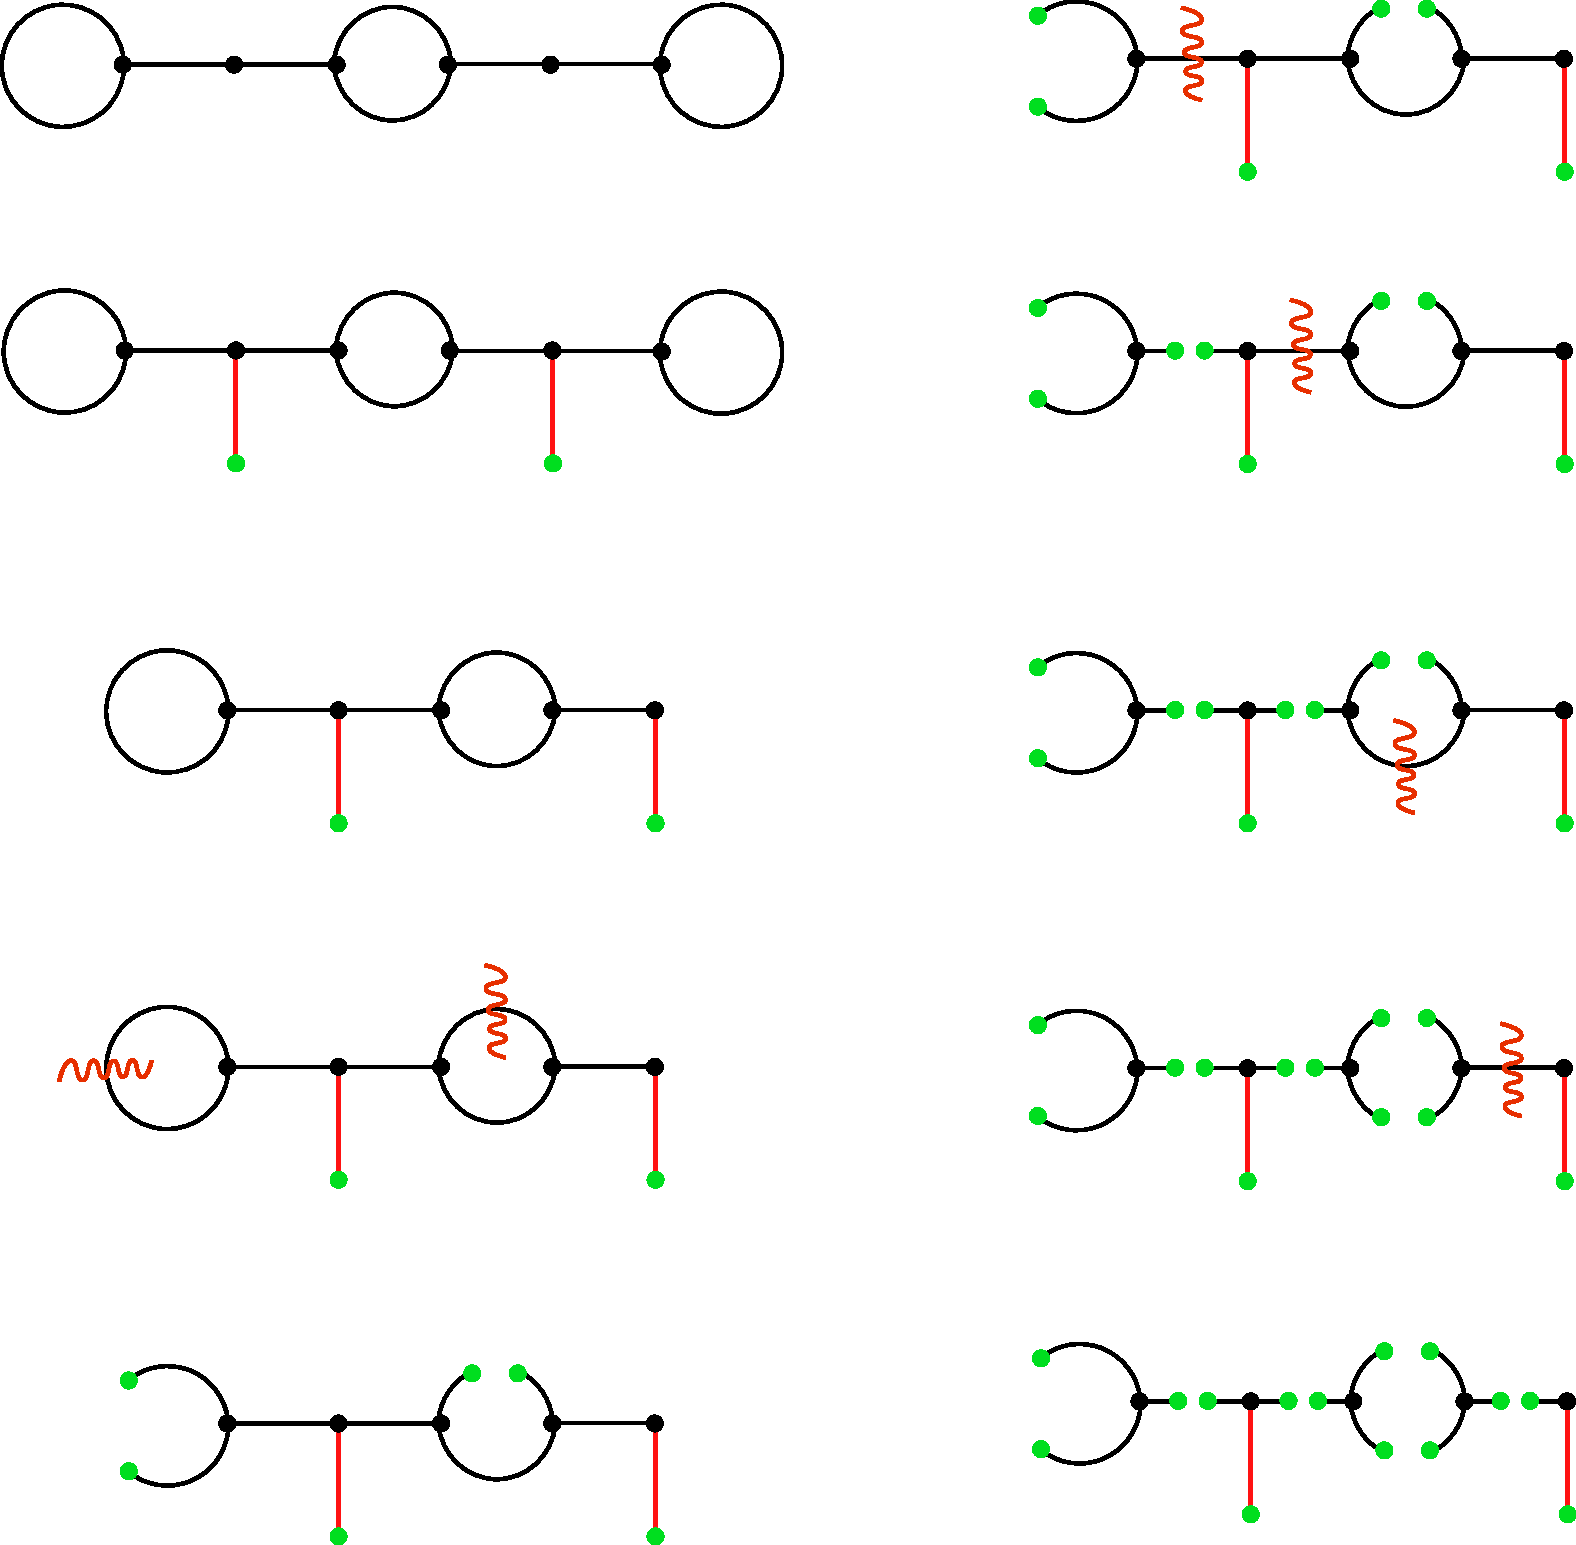
\includegraphics[width=11cm]{Chapter2/Figs/Graphs_Of_Pants}
		\caption{Finding the decomposition $\Gamma$}
		\label{fig:Gen}
	\end{figure}
	
	\begin{figure}[h]
            \centering
		\includegraphics[width=11cm]{Chapter2/Figs/decomp}
		\caption{Pair of pants decomposition corresponding to $\Gamma$}
		\label{fig:Gen}
	\end{figure} 
	Let $\Gamma$ be a graph as described in the statement. 
	\begin{enumerate}
		\item We form a new graph $\Gamma^\prime$ by adding edges to $\Gamma$ at vertices with degree strictly less than 3 and then remove a one-edge loop and the edge connected to its vertex.
		\item Color the new vertices of newly formed edges green. We call them the boundary components. Number these green vertices from $1$ to $n$.
		\item Now, there exists $g-1$ edges, that could be cut off from $\Gamma$ without disconnecting it. Cut these edges in half and color the newly formed vertices green.
		\item Number these green vertices from $n+1$ to $g+n$ such that vertices formed from the same edge gets the same number.
		\item As, there are now $2g-2+n-1$ black vertices and $2g-2+n$ green vertices, there exists a black vertex which has two edges with green vertices. Call this vertex $v$ and let the labels on the green vertices be $r,s$.
		\item Cut the third edge of $v$ in half, adding a new green vertex, say $t$. Now, the graph has $2g-2+n-2$ black vertices and $2g-2+n-1$ green vertices. 
		\item To get the decomposition of our choice, i.e., corresponding to the graph $\Gamma$, we need a choice of boundary components of the torus we started with. For that purpose, identify the green vertices of the graph $\Gamma$ with the boundary components of the torus.   
		\item Proceed with the step described in \cite[Section 5.1-5.6]{GKM} with $r,s$ being the pair of peripheral curves. Thus, we cut off a curve $t$ that bounds $r$ and $s$.
		\item Repeating the argument, we end up atlast with one vertex with two boundary components. Now, we proceed with the step described in \cite[Section 5.7]{GKM} to finish the process.
	\end{enumerate} 

\end{proof}